\chapter{Aktueller Stand der Performance Analyse in der \acl{CE}}
In der \ac{CE} werden bereits verschiedene Wege genutzt, um die Performance und
das Verhalten der HANA Datenbank zu analysieren. 
\section{Google Benchmark}
\label{sec:google_benchmark}

Google Benchmark ist ein Open Source Benchmarking Tool von Google,
welches es einem ermöglicht einzelne Funktionen in C++ zu benchmarken. 
Dazu kann man ähnlich zu den meisten Test Frameworks drei verschiedene
Codeabschnitte definieren.

Der Hauptabschnitt definiert was genau im Benchmark untersucht werden
soll. Diese legt die für die Messung relevante Logik fest.

Der Setup Abschnitt wird einmal vor jeder Ausführung des Benchmarks
aufgerufen. In dieser werden die Voraussetzungen für die Ausführung des Hauptabschnitts
geschaffen. Man könnte sie beispielsweise nutzen, um Testdaten für den Benchmark
zu generieren oder zu laden, da er nicht bei den Messungen beachtet wird.

Der Teardown Abschnitt wird nach jeder Ausführung des Benchmarks aufgerufen.
Dieser beeinflusst, wie der Setup Abschnitt, die Messung nicht.

Des Weiteren bietet Google Benchmark die Option, einen Benchmark mehrmals mit
unterschiedlichen Parametern durchzuführen. Um beispielsweise die Auswirkung
der Größe des Testdatensatzes auf das Ergebnis zu beobachten.

\autoref{fig:google_benchmark_ausgabe} zeigt eine Beispielhafte Google
Benchmark Ausgabe. Benchmark ist dabei der Name des Benchmarks und hinter dem
Schrägstrich die Größe des Inputs. Time ist die durchschnittliche Dauer einer
Ausführung des Hauptabschnitts über alle Iterationen hinweg. CPU ist die
durchschnittliche CPU Zeit einer Ausführung des Hauptabschnitts über alle
Iterationen hinweg. Iterations ist die Anzahl der durchgeführten Iterationen
des Hauptabschnitts, bis ein stabiler Durchschnittswert erreicht wurde.
\autocite[Vgl.][]{GoogleBenchmark}

\begin{figure}[h]
    \begin{center}
        \begin{verbatim}

---------------------------------------------------------------
Benchmark                          Time         CPU Iterations 
---------------------------------------------------------------
BM_RemoveDetachedNodes/2           4 us        4 us     189823 
BM_RemoveDetachedNodes/8           9 us        9 us      78165 
BM_RemoveDetachedNodes/64         58 us       58 us      12106 
BM_RemoveDetachedNodes/512       469 us      468 us       1515 
BM_RemoveDetachedNodes/4096     4237 us     4234 us        166 
BM_RemoveDetachedNodes/8192    10026 us    10019 us         60 
        \end{verbatim}
    \end{center}
    \caption{Google Benchmark Ausgabe}\label{fig:google_benchmark_ausgabe}
\end{figure}

Google Benchmark wird in der \ac{CE} meistens genutzt, um das Verhalten der
Laufzeit bestimmter Funktionen in künstlich generierten Testfällen zu
vergleichen. Hierbei wird jedoch keine HANA Instanz benötigt, da
keine Operationen auf einer Datenbank ausgeführt werden. Es werden folglich
auch keine Testdatensätze für die Datenbank benötigt, sondern nur Daten, auf
welchen man die zu analysierende Methode aufrufen kann. Solche Performance
Tests sind also im Vergleich zu Tests, welche auf eine HANA Instanz mit
Testdatensätzen zugreifen, relativ einfach. Da sie sich weniger Voraussetzungen
haben, und nur auf einen kleinen Teil der Logik fokussiert sind.

\section{HANA Profiler}
\label{sec:hana_profiler}


Eine weitere Methode die Performance und das Verhalten von Software zu
analysieren ist, das bereits in \autoref{sec:types_of_perf_analysis}
beschriebene, Profiling. In der \ac{CE} wird ein eigener Profiler verwendet.
Auf diesen kann entweder manuell oder im Code zugegriffen werden. Dabei sind
die wichtigsten Befehle \texttt{profiler clear} um die aktuellen
Profilinginformationen zurückzusetzen,  \texttt{profiler start} um den Profiler
zu starten, \texttt{profiler stop} um den Profiler zu stoppen und
\texttt{profiler print} um die gesammelten Profilinginformationen auszugeben.

\begin{definition}
    Ein gerichteter Graph ist ein Tupel $G=(V,E)$. $V$ heißt Menge der Knoten.
    $E$ heißt Menge der gerichteten Kanten. Es gilt $V\ne\emptyset$ und $E \subset V \times
    V \setminus \{(v,v) | v \in V\}$. Zwischen zwei Knoten $u,v \in V$ gibt es
    eine Kante mit dem Anfangspunkt $u$ und dem Endpunkt $v$, wenn $(u,v) \in E$.
    Ein Pfad $P$ in $G$  ist eine Folge von Knoten $v_0, \dots ,v_n$. Dabei
    muss $\forall i \in \{0, \dots, n-1 \} : (v_i,v_{i+1}) \in E$ gelten. $v_0$
    heißt Anfangspunkt von $P$, $v_n$ heißt Endpunkt von $P$ und $n$ heißt
    Länge von $P$. Ein Pfad heißt geschlossen, wenn $v_0 = v_n$. Ein
    geschlossener Pfad heißt einfach, wenn $\forall i,j \in \{0,\dots,n-1\}, i
    \ne j:v_i \ne v_j$ gilt. In einem gerichteten Graphen heißt ein einfach
    geschlossener Pfad mit $n\geq 2$ auch Zyklus. Ein Graph heißt azyklisch,
    wenn er keine Zyklen besitzt \autocite[Vgl.][S.221ff]{AlgorithmenUndDatenstrukturen}.
    $G$ heißt gewichtet, wenn es eine Abbildung $g:E\rightarrow \mathbb{R}$
    gibt, welche jeder Kante ein Gewicht zuordnet. Für $e\in E$ heißt $g(e)$
    Gewicht von $e$ \autocite[Vgl.][S.253]{AlgorithmenUndDatenstrukturen}.
    Für zwei Knoten $c$ und $p$ gilt, $c$ ist Kindknoten von $p$, wenn $(p,c)\in V$.
    Umgekehrt gilt, wenn $(p,c)\in V$, $p$ ist Elternknoten von $c$.
    $c$ ist Subknoten von $p$, wenn $\exists P: (v_0=p) \land (v_n=c)$.
    \label{def:graph}
\end{definition}

Die Ausgabe erzeugt dabei ist dabei zwei gewichtete gerichtete azyklische
Graphen, nach \autoref{def:graph}, von denen einer die Verteilung der CPU-Zeit und der andere die
Verteilung der Wartezeit, der aufgerufenen Funktionen beinhaltet. Im Folgenden
werden die beiden Graphen CPU-Graph und Warte-Graph genannt.
\autoref{fig:beispielausgabe_hana_profiler} stellt eine mögliche Ausgabe des
HANA Profilers dar. Die folgende Beschreibung gilt für den CPU- als auch den
Warte-Graphen. Jeder Knoten des Graphen spiegelt eine zur Laufzeit des
Profilers aufgerufene Funktion wider. Jeder Knoten beinhaltet drei
Informationen. Den Namen der aufgerufenen Funktion, sowie den Wert $I$ und den
Wert $E$. $I$ ist der Anteil der Gesamtzeit, welcher von diesem Knoten und all
seinen Subknoten benötigt wurde. $E$ ist der Anteil der Gesamtzeit, welcher
von diesem Knoten benötigt wurde. Folglich gilt für alle Knoten $I\geq E$.
Die Kindknoten eines Knoten $K$ sind die Funktionen, welche von $K$ aufgerufen
wurden.
\begin{figure}[h]
    \begin{center}
        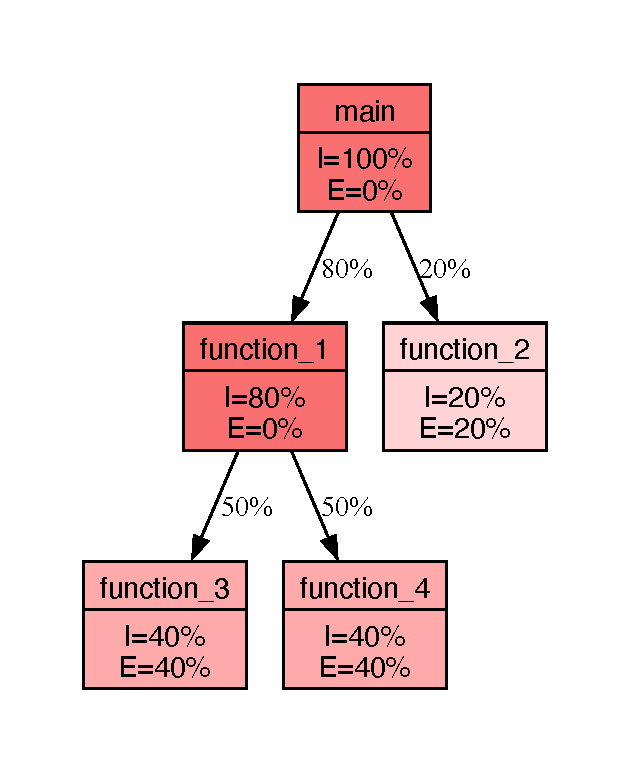
\includegraphics[page=1]{Bilder/pdf/profiler_output_example.pdf}
    \end{center}
    \caption{Beispielausgabe des HANA Profilers}\label{fig:beispielausgabe_hana_profiler}
\end{figure}

